\documentclass{beamer}


\usetheme[progressbar=frametitle]{metropolis}
\usepackage{appendixnumberbeamer}

\usepackage{booktabs}
\usepackage[scale=2]{ccicons}
\usepackage{textpos}
\usepackage{xcolor,colortbl}
\usepackage{pgfplots}
\usepgfplotslibrary{dateplot}
\usepackage{url}
\usepackage[utf8]{inputenc}
\usepackage[T1]{fontenc}
\usepackage{tikzstyles}
\usepackage{textcomp}
\usepackage{pgfplots}
\usepackage{ulem}
\pgfplotsset{compat=1.14}
\usepackage{subfigure} 
\usepackage{mathabx}

\usepackage[
	backend=biber,
	citestyle=authoryear,
	bibstyle=authoryear,
	maxnames=2]{biblatex}
	\bibliography{bibliography.bib}

\usepackage{caption}
\captionsetup{font=scriptsize,labelfont=scriptsize}

% Math symbols
\newcommand{\E}{\mathbb{E}}
\newcommand{\Var}{\mathrm{Var}}
\newcommand{\Cov}{\mathrm{Cov}}

\newcommand\independent{\protect\mathpalette{\protect\independenT}{\perp}}
\def\independenT#1#2{\mathrel{\rlap{$#1#2$}\mkern2mu{#1#2}}}
\DeclareMathOperator*{\argmax}{arg\,max}

\tikzset{
  block/.style    = {draw, thick, rectangle, minimum height = 3em, minimum width = 3em},
  causalvar/.style      = {draw, circle, node distance = 2cm}
}

% Criteo colors/template (legacy)
\definecolor{criteoOrange}{RGB}{248,152,29}

% New names
\definecolor{cOrange}{RGB}{248,152,29}
\definecolor{cBlue}{RGB}{43,46,173}
\definecolor{cGreen}{RGB}{20,171,103}
\definecolor{cRed}{RGB}{248,88,29}

\setbeamercolor{structure}{fg=cOrange,bg=white}
\usepackage{helvet}
\setbeamertemplate{blocks}[rounded]

% https://www.overleaf.com/latex/templates/metropolis-beamer-theme/qzyvdhrntfmr
\addtobeamertemplate{frametitle}{}{%
\textblockcolour{white}
\begin{textblock*}{100mm}(.825\textwidth,-1.08cm)%.825\textwidth,,-1cm)

\includegraphics[scale=.205]{CAIL_logo}%0.3
\end{textblock*}}

\setbeamerfont{normal text}{size=\small}

\title{Face Recognition}

\author{Thomas Ricatte}

\begin{document}

\begin{frame} 	 
\titlepage
\end{frame}

\begin{frame}[fragile]{Outline}
  \tableofcontents
\end{frame}

\section{Motivation}

\begin{frame}{Face Recognition}
\textbf{Objective:} be able to recognize people in multiple environments and conditions (pose, illumination, \dots)
\begin{columns}
\begin{column}{0.5\textwidth}
\textbf{Mainly two tasks}
   \begin{itemize}
       \item \textcolor{cBlue}{Face Verification}~\\
       \textit{Given a photo, find the corresponding person from an input set}
       \item \textcolor{cBlue}{Pair Matching}~\\
       \textit{Determine if a pair of pictures matches or not}
   \end{itemize}
\end{column}
\begin{column}{0.5\textwidth}
    \begin{center}
     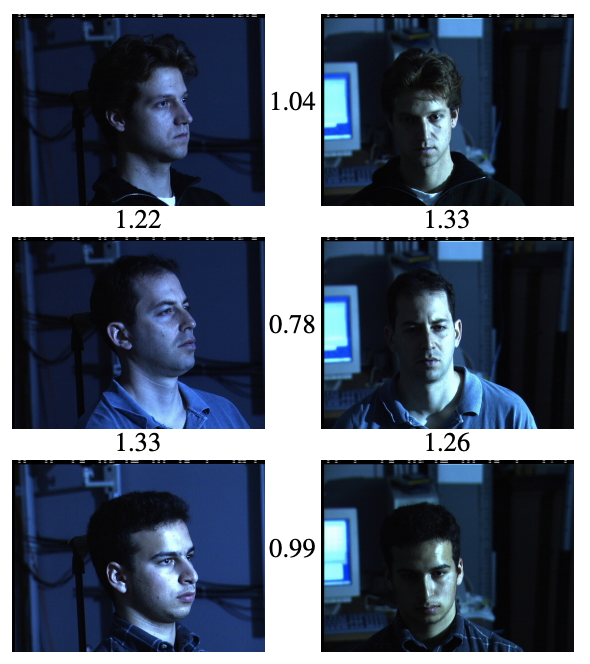
\includegraphics[width=0.8\textwidth]{images/faces.png}
     \end{center}
\end{column}
\end{columns}
\end{frame}

\begin{frame}{Challenges}

{\Large
\begin{enumerate}
    \item \textcolor{cBlue}{Method}: We need to design a training method to solve the above tasks
    \item  \textcolor{cBlue}{Architecture}: We need a model able to extract robust features from the pictures~\\~\\
\end{enumerate}
}

\end{frame}

\begin{frame}{Side note on datasets}

\textbf{Two main public datasets used in papers}
\begin{itemize}
    \item \textbf{LFW (Labeled Faces in the Wild)}~\\
        (\cite{huang2008labeled})~\\
        13k pictures ; 5.7k individuals~\\
        Several protocols: \textit{Restricted / Unrestricted / Unsupervised}
    \item \textbf{YTF (Youtube Faces)}~\\
    (\cite{wolf2011face})~\\
    3.4k videos ; 1.6k individuals
\end{itemize}
% TODO: Evolution of baselines
\end{frame}

\section{Method}

\begin{frame}{Simple classification version}
    \begin{itemize}
        \item First solution is to consider the problem as a multi-class classification problem
        \item The objective is to classify an input picture among a set of $n$ identities $\{ y_1, \dots, y_n \}$
        \item \textbf{Issue:} Mainly a transductive approach. How to generalize to new faces ?
    \end{itemize}
    
    Bottleneck layer ?
    \cite{taigman2014deepface, sun2015deeply}
\end{frame}

\begin{frame}{Pairwise Ranking Loss}
\begin{itemize}
    \item Let's go back to the original problem: classification was just a proxy ! And we need an inductive approach !
    \item \textbf{Idea:} Consider labeled pairs of images for the training (see e.g. \cite{schroff2015facenet})
        \begin{itemize}
            \item Positive: both faces belong to the same persons
            \item Negative: both faces belong to different persons
        \end{itemize}
    \item \textbf{Pairwise loss}~\\
    For a pair of sample $(x_a, x_b)$,
    \[ \mathcal{L}_\theta(x_a, x_b) = \left\lbrace 
    \begin{aligned}
        &d(f_\theta(x_a), f_\theta(x_b))&\text{if positive pair}\\
        &max(0, m-d(f_\theta(x_a), f_\theta(x_b)))&\text{if negative pair}
    \end{aligned} \right.
    \;\;, \]
    where $d$ is a fixed distance function and $m\in \mathbb{R}^+$ an hyperparameter (margin). 
\end{itemize}
\end{frame}
    
\begin{frame}{Siamese Networks}
\begin{itemize}
    \item Note that in the previous slide, $f_\theta$ appears twice in the loss
    \item To implement this, we can use a \emph{Siamese network} 
\begin{figure}
    \centering
    \begin{tikzpicture}
        \draw (-1.2, 0.5) node{$x_a$};
        \draw[->] (-0.8, 0.5) -- (-0.2, 0.5);
        \draw[fill=cBlue!20] (0,0) -- (0,1) -- (1, 1) -- (1, 0) -- (0,0);
        \draw (0.5, 0.5) node{$f_\theta$};
        
        \draw (-1.2, -1) node{$x_b$};
        \draw[->] (-0.8, -1) -- (-0.2, -1);
        \draw[fill=cBlue!20] (0,-1.5) -- (0,-0.5) -- (1, -0.5) -- (1, -1.5) -- (0,-1.5);
        \draw (0.5, -1) node{$f_\theta$};
        
        \draw[->] (1.2, 0.5) -- (3, -0.25);
        \draw[->] (1.2, -1) -- (3, -0.25);
        
        \draw[fill=cBlue!20] (3.2,-0.75) -- (3.2,0.25) -- (4.2, 0.25) -- (4.2, -0.75) -- (3.2,-0.75);
        \draw (3.7, -0.25) node{$d$};
        
        \draw[->] (4.5, -0.25) -- (5.5, -0.25);
    \end{tikzpicture}
\end{figure}
\item $f_\theta$ allows us to perform inductive analysis of new identities.
\end{itemize}
\end{frame}
    


\begin{frame}{“Jamais deux sans trois“}
\begin{itemize}
    \item Other solution is to consider triplets of points
    \begin{itemize}
        \item $x_a$ (anchor): Face of a person 1 
        \item $x_p$ (positive): Another face of person 1
        \item $x_n$ (negative): Face of person 2
    \end{itemize}
    \item We basically want $f_\theta$ such that
    \[ d(f_\theta(x_a), f_\theta(x_p))<d(f_\theta(x_a), f_\theta(x_n)) \;\;.\]
    \item Hence
    \[
    \mathcal{L}_\theta(x_a, x_p, x_n) = 
    max(0, m + d(f_\theta(x_a), f_\theta(x_p)) - d(f_\theta(x_a), f_\theta(x_n))) \;\;,
    \]
    with $m\in \mathbb{R}^+$.
    \item Siamese networks $\to$ Triplets networks
\end{itemize}
\end{frame}

\begin{frame}{How to select triplets ?}
\begin{itemize}
    \item Bad triplet $\to \mathcal{L}_\theta = 0$ 
    \item Selecting a good triplet is important !
    \begin{itemize}
        \item Hard positive: aka $d(f_\theta(x_a), f_\theta(x_p))$ is big
        \item Hard negative: aka $d(f_\theta(x_a), f_\theta(x_n))$ is small
    \end{itemize}
    \item Two approaches
        \begin{itemize}
            \item Offline: every $n$ steps, do argmin / argmax on the full dataset
            \item Online: Do argmin / argmax on each mini-batch
        \end{itemize}
    \item Usually online approach is more efficient (see \cite{schroff2015facenet})
\end{itemize}
\end{frame}

\section{Architecture}

\begin{frame}{3D Alignment (\cite{taigman2014deepface})}

    \begin{itemize}
        \item Analytical m3D model
        \item Similar fiducial points
        \item Similarity transformation (unsupervised)
    \end{itemize}
\end{frame}



\section*{References}

\begin{frame}[allowframebreaks]\small
  \frametitle{References}
  \renewcommand*{\bibfont}{\footnotesize}
  \printbibliography
\end{frame}

\end{document}
